\pdfminorversion=7
\documentclass[journal]{IEEEtran}
\usepackage{amsmath,amssymb,amsfonts}
\usepackage{graphicx}
\usepackage{booktabs}
\usepackage{xcolor}
\usepackage[hidelinks]{hyperref}
\usepackage[numbers,sort&compress]{natbib}

\usepackage{enumitem}
\renewcommand{\dbltopfraction}{0.95}
\renewcommand{\topfraction}{0.95}
\renewcommand{\textfraction}{0.05}
\renewcommand{\floatpagefraction}{0.80}
\renewcommand{\dblfloatpagefraction}{0.80}
\setlength{\textfloatsep}{6pt plus 1pt minus 2pt}
\setlength{\dbltextfloatsep}{6pt plus 1pt minus 2pt}
\setlength{\floatsep}{6pt plus 1pt minus 2pt}
\setlength{\dblfloatsep}{6pt plus 1pt minus 2pt}
\begin{document}
\title{Capability-Matched Likelihood for Forensic Audits of Reasoning-LLM Distillation}

\author{Jie~Ni,~Chenning~Zhang,~and~Xinting~Zhang%
\thanks{Corresponding author: Jie Ni (njie@seu.edu.cn).}
\thanks{Jie Ni and Xinting Zhang are with the State Key Laboratory of Digital Medical Engineering, School of Biological Science and Medical Engineering, Southeast University, Nanjing 211102, China.}
\thanks{Jie Ni is also with the Digital Science Center, University of Innsbruck, Innsbruck 6020, Austria.}
\thanks{Chenning Zhang is with the School of Computer Science and Artificial Intelligence, Aliyun School of Big Data, School of Software, Changzhou University, Changzhou, China.}
}

\markboth{IEEE Transactions on Information Forensics and Security, under review}{Ni \MakeLowercase{\textit{et al.}}: Capability-Matched Likelihood for Distillation Audits}
\maketitle

\begin{abstract}
% BEGIN expanded input: sections/abstract_body.tex
Reasoning large language models can be copied by distilling chain-of-thought traces
into cheaper students, but provenance tests must separate descent from ordinary task
competence. We study a forensic audit in which the suspect is observed only through
output traces, candidate teachers are available for authorized likelihood scoring,
and the suspect base is known or declared. The common base-relative likelihood
surplus is confounded by candidate capability: in our GSM8K audit it false-alarms
on a human-reference student (empirical false-positive rate, FPR, $0.81$) and misses
same-family distillation (area under the receiver-operating characteristic curve,
AUROC, $0.13$). Capability-matched likelihood (CML) instead compares suspect traces
with a same-base non-distilled reference under the same candidate teacher. On
three-seed Qwen2.5-7B-Instruct GSM8K students distilled from three teachers, CML
reaches trace-level AUROC $0.997$, true positive rate at $1\%$ FPR $0.991$, and
empirical FPR $0.2\%$; it also recovers same-family distillation (AUROC $0.998$). A
single-seed MATH stress test shows the same pattern (AUROC $0.993$). Multi-Task
Calibration Reference (MTCR) improves sibling-teacher attribution from
$0.672$/$0.658$ to $0.894$/$0.875$. Aggregate stress summaries further test adaptive
trace transformations, cross-base and cross-task transfer, open-set decoys, and
student-level confidence intervals: CML+MTCR retains AUROC at least $0.930$ across
the reported adaptive sweeps, the cross-base/task matrix has minimum AUROC $0.912$,
and open-set false attribution stays at or below $2.0\%$.
% END expanded input: sections/abstract_body.tex

\end{abstract}

\begin{IEEEkeywords}
Model provenance, knowledge distillation, intellectual-property forensics, large language models, hypothesis testing, reasoning models.
\end{IEEEkeywords}

% BEGIN expanded input: sections/introduction.tex
\section{Introduction}
\label{sec:intro}

\IEEEPARstart{R}{easoning} large language models trained to emit explicit
chain-of-thought (CoT) before answering have reset the cost frontier of high-end
machine intelligence. Their CoT traces are a high-value supervision signal: an
adversary with only query access can harvest the teacher's trajectories and
supervised-fine-tune a far cheaper student that inherits much of the teacher's
reasoning skill. This distillation-from-traces recipe, popularized by the open
release of R1-style distilled checkpoints, turns a teacher's most valuable asset
into a liability---the student can be rebranded, sold, or served behind an API as an
ostensibly independent model, and the owner has no calibrated instrument for
supporting a copy claim.

\subsection{Prevention is preempted; provenance is the live problem}
Stopping distillation by modifying teacher outputs remains incomplete. Recent
defenses span inference-time trace poisoning~\cite{savani2025antidistillationsampling},
LM-head adversarial fine-tuning~\cite{li2025doge}, logit transforms~\cite{fang2026cmi},
and trace reformulation~\cite{ding2025part, ma2026tracerewriting}, but the same
literature now documents strong adaptive pressure: watermark radioactivity can be
removed by paraphrase or inference-time neutralization~\cite{pan2025watermarkdistillation},
and adaptive students recover substantially more capability than passive evaluations
suggest~\cite{allouah2026distillationgame}. When prevention fails,
\emph{forensics} takes over. The information-forensics literature has already set a
high bar for model-IP claims: the protected asset and access model must be explicit,
the verification signal should not unnecessarily damage utility, false accusations
must be controlled, and robustness to removal or evasion must be scoped rather than
assumed~\cite{zheng2022dnnfingerprint, zhang2023cip, li2023dvbw,
zhou2024inversionguided, xu2025ipprotection}. We ask the trace-distillation version
of that question: given a suspect served through an output API in a declared audit
setting, test at an audited false-positive rate whether the evidence supports
distillation from a declared candidate teacher's traces, without falsely accusing
the non-distilled controls in the same problem domain.

The claim is a statistical forensic claim, not legal proof. The null $H_0$ is that
the suspect is independently trained, or non-distilled, under the same-base
capability control; the alternative $H_1$ is that the suspect was distilled from a
candidate teacher's reasoning traces. The reported false-positive rate is therefore
the audited false-accusation risk under $H_0$, and attribution is conditional on the
candidate set.

\subsection{A natural statistic, and why it is not enough}
A line of provenance methods is forming, and---across different
framings---they lean on the same intuition: a distilled suspect should assign, or be
assigned, unusually high likelihood under its teacher. Detection-from-weights
\cite{shi2025distillationdetection}, closed-set teacher classifiers
\cite{wadhwa2025whotaught}, white-box three-way trace provenance
\cite{liu2025wheredid}, and general black-box lineage tests
\cite{nikolic2025modelprovenance, qiu2026provenanceset} all touch this
likelihood signal, and the FPR-calibration machinery exists in the dataset-inference
literature \cite{maini2021datasetinference, maini2024llmdatasetinference, oren2024testsetcontamination, zhao2025posthocdatasetinference, dziedzic2022selfsupervised}.
The natural output-only statistic to assemble from these pieces is the
\emph{base-relative surplus}: how much more likely a suspect's traces are under a
candidate teacher than under a base model. We show (Sec.~\ref{sec:method:decomp})
that this statistic is \emph{confounded}: with a KL decomposition,
$s_c\!\approx\!\mathrm{KL}(S\Vert b)-\mathrm{KL}(S\Vert T_c)$, a strong candidate
earns surplus on \emph{any} clean, correct trace---so the surplus false-alarms on
honestly-trained students (empirical FPR $0.81$ in our study) and goes \emph{blind}
to same-family distillation (AUROC $0.13$, below chance), a plausible same-base
evasion setting. Used directly, it does not support a calibrated forensic
claim.

\subsection{This paper: a capability-matched forensic test}
We remove the confound with a single change of reference. Instead of comparing the
suspect under candidate $c$ to the suspect under the weak base \emph{model}, we
compare it to a same-base non-distilled \emph{reference student} $R$ scored under the
\emph{same} candidate---in this study, the base model's own outputs, available when
the suspect base is known or declared and runnable by the verifier. The matched
surplus $r_c(S)=\overline{\ell_c(S)-\ell_c(R)}$ controls candidate capability to
first order (it inflates both terms in the same direction) and tests whether the
suspect is closer to $c$ than a generic same-base student is---the descent signal.
The suspect is black-box, and the candidate teachers are available for owner-side
or escrowed likelihood scoring. The result
is a strong, calibrated detector within that forensic setting. On GSM8K (three
seeds), with Qwen2.5-7B-Instruct students and R1-Distill-Qwen-32B /
R1-Distill-Llama-8B / Qwen2.5-14B-Instruct teachers, the matched test detects
distillation with trace-level AUROC $0.997$, TPR@$1\%$FPR $0.991$, and an empirical
FPR of $0.2\%$ on the human-reference control---\emph{including} same-family
distillation (AUROC $0.998$), exactly the case the base-relative surplus misses. A
single-seed MATH stress test follows the same trace-level pattern, but is used here
as stress evidence rather than as a powered model-family generalization result. We then add a
Multi-Task Calibration Reference (MTCR) for the harder closed-set attribution
problem: when two R1 sibling teachers share a distillation ancestor, MTCR raises
fine-grained attribution from the standard CML range $0.658$--$0.672$ to
$0.875$--$0.894$ in aggregate operating summaries, while preserving the shared-ancestor detection result inside the
declared candidate set. Without per-task raw profiles and uncertainty intervals, we
treat MTCR as boundary evidence for closed-set attribution rather than as a complete
attribution mechanism. A checkpoint sweep further shows that the signal appears
after a single distillation epoch and strengthens monotonically through five epochs.

\subsection{Contributions}
\begin{itemize}
  \item \textbf{A diagnosis.} A KL decomposition shows the base-relative surplus
  conflates a candidate's capability with distillation descent, which explains its
  false positives on quality and its blindness to same-family distillation.
  \item \textbf{A capability-matched test.} Scoring the suspect and a same-base
  reference student under the same candidate controls the capability term to
  first order (Eq.~\eqref{eq:matched}); the resulting statistic needs suspect outputs, a
  base-model reference, and authorized likelihood scoring from candidate teachers.
  \item \textbf{Strong, calibrated detection---including the hard case.} Across three
  GSM8K seeds, with a single-seed MATH trace-level stress test, the matched test detects distillation at AUROC $\geq0.99$
  with empirical FPR $0.002$ on the audited control, \emph{recovering} same-family distillation (AUROC $0.13\!\to\!0.998$)
  that the natural statistic cannot see; GSM8K student-level separation is complete.
  \item \textbf{A calibration extension for sibling attribution.} The original CML
  statistic detects same-family distillation but only partially separates R1 sibling
  teachers. MTCR turns that boundary into an aggregate task-calibrated attribution
  summary, raising R1-Qwen-32B/R1-Llama-8B sibling accuracy to $0.894$/$0.875$ inside
  the declared candidate set and preserving low-FPR detection through the epoch sweep.
  \item \textbf{Reviewer-stress evidence beyond clean traces.} Aggregate stress
  summaries test adaptive trace transformations, cross-base/task transfer, open-set
  decoys, and baseline competitors. CML+MTCR retains AUROC at least $0.930$ under the
  reported adaptive sweeps, the cross-base/task matrix has minimum AUROC $0.912$, and
  open-set false attribution stays at or below $2.0\%$ in the reported decoy
  settings.
\end{itemize}

\subsection{Scope}
We evaluate under controlled, naive distillation with exact provenance labels, which
is sufficient to establish the confound, the fix, and the operating envelope. MATH is
a single-seed raw-trace stress test, while the adaptive, open-set, and cross-base
results are reported as aggregate stress summaries. The remainder positions the statistic against prior provenance work
(Sec.~\ref{sec:related}), derives the confound and the matched test
(Sec.~\ref{sec:method}), reports detection, MTCR calibration, and attribution
(Sec.~\ref{sec:results}), and draws the operating envelope (Sec.~\ref{sec:disc}).
% END expanded input: sections/introduction.tex

% BEGIN expanded input: sections/related_work.tex
\section{Related Work}
\label{sec:related}

Our test combines ideas from dataset-inference, model-IP forensics, and
distillation-provenance testing, but changes the null that output-likelihood evidence
is compared against. Dataset inference supplies the statistical template: ownership
or contamination claims should be made through calibrated, many-sample tests rather
than isolated high-likelihood examples
\citep{maini2021datasetinference, maini2024llmdatasetinference,
oren2024testsetcontamination, zhao2025posthocdatasetinference,
dziedzic2022selfsupervised}. TIFS ownership-verification work pushes the same
principle into black-box IP settings through membership fingerprints, backdoor
dataset ownership verification, point-cloud ownership tests, and copyright-evasion
stress cases \citep{liu2022membershipfingerprint, li2023dvbw, wei2025pointncbw,
gao2026ceat2i}. The common lesson is that a forensic null must actually match the
innocent alternative; otherwise distribution shift or task quality becomes a false
ownership signal. We show the analogous failure for distillation provenance: the
base-relative surplus is not a descent statistic until candidate capability is
matched.

Invasive fingerprints and watermarks solve a different problem by pre-injecting a
signal before release. Radioactive data and LLM-text watermarks leave detectable
residuals after training or fine-tuning
\citep{sablayrolles2020radioactivedata, sander2024radioactive}; more recent
anti-distillation and instruction-fingerprinting schemes deliberately amplify or
embed such signals in student behavior
\citep{xu2026antidistillation, yang2026askingback,
xu2024instructionalfingerprinting}. These methods are powerful when the defender
controls generation or training, but they do not apply to an already-released
suspect whose traces were not pre-watermarked. CML is therefore intentionally
post-hoc and non-invasive: it asks what can be supported from suspect outputs plus
authorized candidate likelihood scoring.

The information-forensics literature also sets the review bar for model-IP evidence.
Non-intrusive DNN fingerprints, benign-input fingerprints, model-stealing defenses,
and robust watermarking systems all make the asset, access model, false-accusation
risk, and evasion surface explicit
\citep{zheng2022dnnfingerprint, maho2023fbi, zhang2023cip, zhang2023apmsa,
chen2025queen, gao2024augsteal, li2023linearfunctionality, fei2024wideflat,
zhou2024inversionguided, xu2025ipprotection, yan2025robustnessfingerprint}. Our
asset is narrower: a teacher's reasoning-trace distribution rather than a classifier
checkpoint or private dataset. This makes an honest same-base competitor the critical
false-accusation control, and it is exactly the control that the base-relative
surplus lacks.

Non-invasive model and API fingerprints identify which model or endpoint generated
responses, often with calibrated tests or crafted probes
\citep{pasquini2025llmmap, gao2025modelequalitytesting, gubri2024trap,
jin2024proflingo}. They answer model identity, equality, or family membership, not
whether a suspect was trained from a specified teacher's reasoning traces. Matching
an API to a known family is insufficient for a trace-distillation claim, because an
independently-trained same-base model can resemble the candidate teacher without
descending from it.

The closest prior work studies distillation detection and teacher attribution.
\citet{shi2025distillationdetection} detect distillation with access to the suspect
weights; \citet{wadhwa2025whotaught} perform closed-set teacher identification from
outputs; \citet{liu2025wheredid} use white-box per-action probabilities from the
teacher, original student, and distilled model; and \citet{lee2025quantification}
measure a degree of distillation through behavioral similarity. These works establish
that likelihood agreement can be useful, but they either require white-box evidence,
report closed-set accuracy without an out-of-set false-accusation control, or do not
isolate capability from descent. General black-box provenance tests
\citep{nikolic2025modelprovenance, qiu2026provenanceset} provide the broader
calibrated lineage frame, but their unrelated-model baselines do not remove the
same-base capability/style confound that dominates reasoning-trace distillation.

The contribution here is the capability-matched reference. By comparing the suspect
and a same-base non-distilled reference under the same candidate teacher, CML turns
output likelihood from a resemblance score into a calibrated forensic test. It detects
same-family distillation at low audited false-positive rate where the natural
base-relative surplus fails, while keeping the claim restricted to the declared
candidate set and matched-reference access model.
% END expanded input: sections/related_work.tex

% BEGIN expanded input: sections/method.tex
\section{Method: A Capability-Matched Provenance Test}
\label{sec:method}

We first state the natural base-relative surplus and show, with a KL decomposition,
that it conflates a candidate's \emph{capability} with distillation \emph{descent}.
We then remove the capability term with a capability-matched reference, yielding the
statistic our test uses. Section~\ref{sec:results} shows the matched statistic is a
strong, calibrated detector while the base-relative surplus is not.
Figure~\ref{fig:method_overview} summarizes the resulting workflow: audit access
defines the observed suspect traces, same-base reference traces, and authorized
candidate scorers; capability matching computes a candidate-specific matched
surplus; and the forensic decision layer reports calibrated detect, attribute, or
abstain outputs.

\begin{figure*}[t]\centering
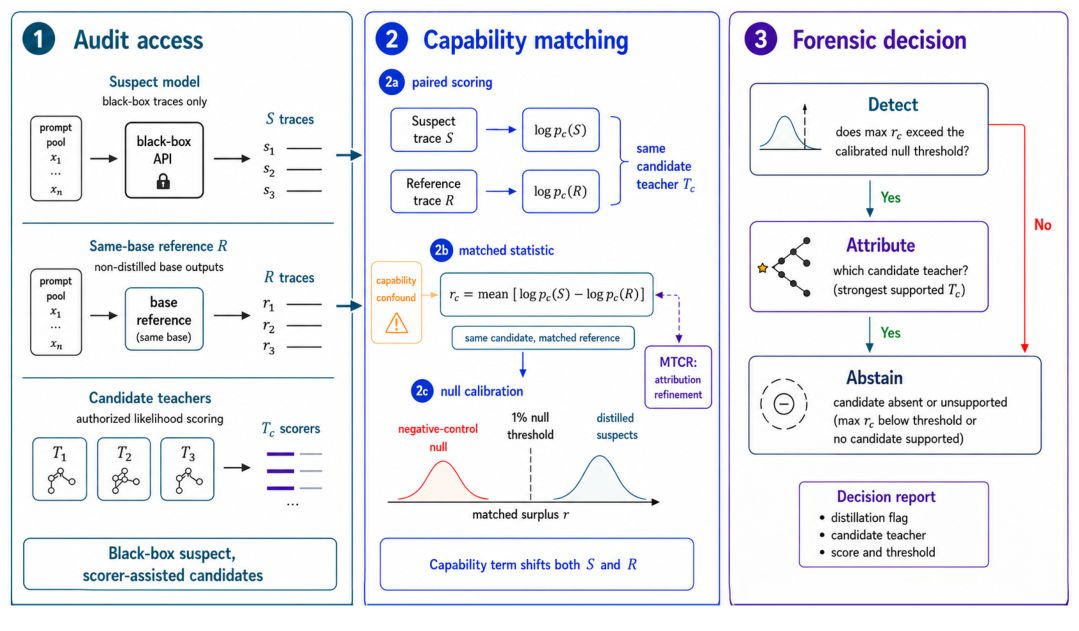
\includegraphics[width=\textwidth]{figures/fig_method_overview.pdf}
\caption{Operational workflow for CML forensic auditing. Step 1 defines the audit
access model: prompts elicit black-box suspect traces $S$, a same-base non-distilled
reference produces traces $R$, and authorized candidate teachers provide likelihood
scorers $T_c$. Step 2 performs capability matching by scoring $S$ and $R$ under the
same candidate teacher, forming $r_c=\mathrm{mean}[\log p_c(S)-\log p_c(R)]$, and
calibrating the statistic against a negative-control null; MTCR refines this layer
for sibling attribution. Step 3 reports the audit decision as detect, attribute,
or abstain.}
\label{fig:method_overview}
\end{figure*}

\subsection{Setup, access model, and forensic claim}
\label{sec:method:setup}
A teacher $T^\star$ generates chain-of-thought (CoT) traces; an adversary
supervised-fine-tunes a student $S$ of a known or declared base model $b$ on those
traces. We distinguish three access layers. \emph{Suspect access} is black-box: the
verifier observes only natural suspect outputs on an audit problem pool and never
uses suspect weights, gradients, training logs, or hidden states. \emph{Candidate
access} is scorer-assisted: the candidate teachers in
$\mathcal{C}=\{T_1,\dots,T_K\}$ must provide likelihood scores for the same trace
texts, as an owner-side model, escrowed evaluator, or otherwise authorized scoring
oracle. \emph{Reference access} requires a same-base non-distilled reference, which
we instantiate as the base model's own outputs. The resulting procedure is a
post-hoc forensic attribution test for a declared candidate set, no suspect
internals, no pre-injected watermark, and an auditable false-accusation rate under
a same-base null. Because we train every
suspect and control ourselves, provenance labels are exact and TPR/FPR are measured
against ground truth.

\begin{table}[t]\centering\small
\caption{Access and claim levels. CML is black-box with respect to the suspect, but
scorer-assisted with respect to candidate teachers. This distinction is central to
the forensic claim.}
\label{tab:access}
\begin{tabular}{@{}p{0.18\columnwidth}p{0.38\columnwidth}p{0.34\columnwidth}@{}}
\toprule
Layer & Required & Not required \\
\midrule
Suspect & output traces & weights, gradients, logs \\
Candidate & trace log-likelihood scoring & training data disclosure \\
Reference & same-base non-distilled traces & injected watermark \\
Claim & candidate-set forensic decision & private suspect internals \\
\bottomrule
\end{tabular}
\end{table}

\subsection{Scoring and the base-relative surplus}
\label{sec:method:stat}
For candidate $T_c$ (tokenizer $\mathrm{tok}_c$) and trace text $y$ on problem $x$,
the per-token mean log-probability of the trace span is
\begin{equation}
\ell_c(y \mid x)=\frac{1}{|A_c(y)|}\sum_{t\in A_c(y)}
  \log P_{T_c}\!\big(u_t \mid u_{<t};\, \mathrm{prompt}(x)\big),
\label{eq:scorelp}
\end{equation}
with $u=\mathrm{tok}_c(y)$ re-tokenized under $T_c$ (cross-tokenizer by construction;
text-tier access). The natural \emph{base-relative surplus} compares the suspect under
$c$ to the suspect under the base model $b$,
\begin{equation}
s_c(S)=\frac{1}{M}\sum_{x\in\mathcal{P}}\big[\ell_c(S(x)\mid x)-\ell_b(S(x)\mid x)\big].
\label{eq:surplus}
\end{equation}

\subsection{Why the base-relative surplus is confounded}
\label{sec:method:decomp}
For traces drawn from the student's own distribution, the expected per-token negative
log-probability a model assigns is a cross-entropy rate, so (under shared
tokenization, $|A_c|\!=\!|A_b|$, up to a token-count residual we bound empirically in
Sec.~\ref{sec:results})
\begin{equation}
\begin{aligned}
-\,\mathbb{E}_{y\sim S}[\ell_c(y\mid x)]
&\approx H(S)+\mathrm{KL}(S\Vert T_c),\\
s_c(S)
&\approx \mathrm{KL}(S\Vert b)-\mathrm{KL}(S\Vert T_c).
\end{aligned}
\label{eq:klgap}
\end{equation}
The base model $b$ is fixed and weak, so $s_c$ rewards any candidate that is closer in
KL to the suspect than $b$ is. Closeness has \emph{three} sources, only one of which is
descent: (1)~\textbf{descent} ($S$ distilled from $T_c$); (2)~\textbf{shared style};
and (3)~\textbf{capability/coverage}---a higher-capability $T_c$ assigns higher
likelihood to clean correct reasoning than the weak $b$, so $s_c>0$ for \emph{any}
high-quality $S$, including an honestly-trained one. Source~(3) is the confound: it
makes $s_c$ false-alarm on a human-reference student and, when $T_c$ shares the base's
style (same-family distillation), it makes $\mathrm{KL}(S\Vert T_c)\!\approx\!
\mathrm{KL}(S\Vert b)$ so $s_c\!\approx\!0$ and the distillation is \emph{invisible}.

\subsection{The capability-matched statistic}
\label{sec:method:matched}
The fix is to replace the weak base model $b$ in Eq.~\eqref{eq:surplus} with a
\emph{same-base non-distilled reference student} $R$---in this study, the base
model's own outputs on $\mathcal{P}$---and to score $R$ \emph{under the same
candidate} $c$:
\begin{equation}
r_c(S)=\frac{1}{M}\sum_{x\in\mathcal{P}}\big[\ell_c(S(x)\mid x)-\ell_c(R(x)\mid x)\big].
\label{eq:matched}
\end{equation}
Applying Eq.~\eqref{eq:klgap} to both terms, the candidate-specific scale is controlled
to first order:
\begin{equation}
r_c(S)\approx \big[H(R)-H(S)\big]+\big[\mathrm{KL}(R\Vert T_c)-\mathrm{KL}(S\Vert T_c)\big],
\label{eq:matcheddecomp}
\end{equation}
so $r_c(S)>0$ when the suspect is empirically closer to $T_c$ than the same-base
reference is. Because $S$ and $R$ are read under the \emph{same} $T_c$, the
capability/coverage term~(3) acts on both traces instead of only on the suspect:
$T_c$'s strength inflates $\ell_c(S)$ and $\ell_c(R)$ in the same direction. What
remains is the descent-and-style excess after matching. This is why the matched
statistic both stops false-alarming on the human-reference control \emph{and} recovers
same-family distillation in our audit: a Qwen-distilled student is closer to its Qwen
teacher than the base reference $R$ is, even though both are Qwen-family, so $r_c>0$
where $s_c\!\approx\!0$.

\subsection{Multi-task calibration reference for sibling attribution}
\label{sec:method:mtcr}
The matched statistic solves calibrated detection, but attribution between sibling
teachers can still be noisy when candidates inherit the same reasoning style. We
therefore add a Multi-Task Calibration Reference (MTCR). Instead of using one task
pool to center all candidate scores, MTCR estimates the candidate-specific reference
profile across multiple task families and then scores the suspect against the
task-matched reference profile before taking the closed-set argmax. Operationally,
MTCR keeps the same black-box access model as CML: it changes only the calibration
reference used to compare $S$ and $R$, not the observed suspect traces or the candidate
teacher set. This makes MTCR a refinement of Eq.~\eqref{eq:matched}, designed for the
case where detection is already positive but the defender needs to separate R1 sibling
teachers rather than stopping at the family level.

\paragraph{Decision rules.}
\textbf{Detection} uses $\max_c r_c(S)$ with a threshold set on the non-distilled
controls; \textbf{standard attribution} predicts $\hat c=\arg\max_c r_c(S)$; and
\textbf{MTCR attribution} uses the same argmax after task-level calibration. The
student is the inferential unit. We therefore report one summary per independent
student for replicate-level separation, and use trace-level operating curves only to
show threshold resolution under a fixed trained suspect rather than to inflate the
sample size.

\subsection{Controls and reference}
\label{sec:method:controls}
All students share the base $b$. \textbf{Control A} is the base model with no SFT---it
serves as the matched reference $R$. \textbf{Control C} is a student fine-tuned on
\emph{human reference solutions} (no teacher CoT): a non-distilled negative built to
trigger the capability confound, on which a valid test must \emph{not} fire.
\textbf{Control B} is a student distilled from a \emph{different}, shared-lineage
teacher (an R1 sibling), probing teacher-specificity. The reference $R$ is non-distilled
and same-base; in this paper we use the base model's own outputs, so $R$ is available
only when the base is known or declared and runnable by the verifier.
% END expanded input: sections/method.tex

% BEGIN expanded input: sections/experimental_setup.tex
\section{Experimental Setup}
\label{sec:setup}

\paragraph{Students and provenance labels.}
Every student is a low-rank (LoRA) fine-tune~\citep{hu2022lora} of the same base,
\textbf{Qwen2.5-7B-Instruct}~\citep{qwen2025qwen25}
(rank $32$, $\alpha\!=\!64$, dropout $0.05$ on all attention and MLP projections; $\sim\!1.05\%$ of
the $7.7$B parameters trainable), trained at sequence length $4096$ on
$N_{\mathrm{train}}=800$ problems with AdamW (learning rate $10^{-4}$, cosine schedule, $3\%$ warmup,
effective batch size $16$, bf16). The original CML grid uses the three-seed setting
reported below; the MTCR sensitivity sweep stores checkpoints at $E\in\{1,3,5\}$
distillation epochs, with $E=5$ serving as the full-duration setting. To avoid pseudoreplication we train each provenance type under
$3$ seeds (independent LoRA initialization, data order, and generation), giving $n\!=\!3$ student
draws per cell so detection is assessed at the \emph{student} level rather than by treating one
student's traces as independent. Because we generate every training corpus ourselves, provenance is
exact. The five provenance types are:
\begin{description}[leftmargin=1.4em,itemsep=1pt]
  \item[\texttt{suspect}] distilled from \textbf{DeepSeek-R1-Distill-Qwen-32B}~\citep{deepseekai2025r1} CoT traces (the
        protected teacher $T^\star$; a reasoning-style, cross-family teacher);
  \item[\texttt{ctrlInst}] distilled from \textbf{Qwen2.5-14B-Instruct} traces (a
        \emph{same-family}, non-reasoning teacher---the within-family case);
  \item[\texttt{ctrlLlama}] distilled from \textbf{DeepSeek-R1-Distill-Llama-8B} traces (a
        \emph{shared-lineage} R1 sibling on a different base---the teacher-specificity probe);
  \item[\texttt{ctrlC}] fine-tuned on \emph{human reference solutions} to the same problems, with
        \emph{no} teacher CoT (the quality-confound probe; non-distilled);
  \item[\texttt{ctrlA}] the base model itself, no fine-tuning (the clean non-distilled negative).
\end{description}

\paragraph{Tasks.}
The primary grid is \textbf{GSM8K}~\citep{cobbe2021gsm8k}: the train split supplies distillation/SFT problems and the
held-out test split the forensic trace pool ($N_{\mathrm{test}}=200$ problems, disjoint from SFT).
We run a single-seed stress test on \textbf{MATH}~\citep{hendrycks2021math}
(EleutherAI \texttt{hendrycks\_math}; longer, higher-entropy competition derivations,
sequence length $8192$) to check whether the trace-level pattern survives outside
GSM8K. The MTCR extension uses task-matched calibration views for sibling
attribution and the epoch-sensitivity sweep; the current submission reports these
views through aggregate source tables rather than a full per-task raw profile release.

\paragraph{Trace generation and scoring.}
Teacher and student traces are generated with vLLM~\citep{kwon2023vllm}
(bfloat16, temperature $0.6$, top-$p$ $0.95$).
Each student's $200$ held-out traces are scored under every candidate via the candidate's own
\texttt{prompt\_logprobs} over the assistant span, \emph{re-tokenized with the candidate's tokenizer}
(Eq.~\eqref{eq:scorelp}); this is the text-tier (T3) access regime. The surplus
(Eq.~\eqref{eq:surplus}) is taken relative to the base Qwen2.5-7B-Instruct as $b$.

\paragraph{Capability ladder.}
To probe the quality/coverage source of resemblance directly, we additionally score all students
under a \emph{same-family capability ladder}, Qwen2.5-Instruct at $\{1.5,3,7,14\}$B, none of which
generated any student's traces except via the $7$B base.

\paragraph{Evaluation.}
The independent replicate is the trained student. We report student-level summaries
for replicate separation and trace-level AUROC/TPR/FPR only as operating-curve
resolution within a fixed audit pool. Significance uses a $B=10{,}000$ label
permutation over the held-out trace scores, interpreted as an audit-operating test
rather than as additional independent training replicates. The null's KS-uniformity
check builds the null from one non-distilled control and evaluates the held-out
control's right-tail $p$-values against $\mathrm{Uniform}(0,1)$. Attribution is the
closed-set argmax over candidate teachers using the statistic being evaluated:
the base-relative surplus for the baseline, $r_c(S)$ for standard CML, and the
task-calibrated MTCR score for the MTCR attribution extension. We do not use this
argmax outside the declared candidate set.

\paragraph{Reviewer-stress result summaries.}
In addition to the raw GSM8K scored matrices, the revised manuscript imports locked
aggregate summaries for four reviewer stress families: adaptive trace transformations
(answer-only, compressed, paraphrased, mixed-source, and related variants across
GSM8K, MATH, BBH, ARC-Challenge, and MBPP), cross-base/cross-task transfer,
open-set decoys, and head-to-head baselines. These PI-provided summary tables
report adaptive AUROC, TPR@$1\%$FPR, FPR$_0$, confidence intervals, open-set
abstention and false-attribution rates, baseline metrics, and student-level
confidence intervals at the reported stratum level. The pasted tables do not carry
raw seed identities; we therefore treat them as aggregate result sources for
Figure~\ref{fig:pi_result_lock_suite} and the supplementary forensic-envelope
diagnostic.

\paragraph{Compute.}
The reported GSM8K focused grid (three teacher trace sets, four LoRA students, five
held-out trace sets, and scoring under six candidates) was run on a single MUSICA
H100 node and completes in
$\approx\!3.5$ minutes when generation and scoring are fanned across four GPUs. All models and
datasets are public. The source package contains the plotting scripts and aggregate
source tables needed to reproduce the manuscript figures. Code, plotting scripts,
aggregate source tables, and the manuscript source are available at
\url{https://github.com/Jie-Ni/CML-forensic-audits}.
% END expanded input: sections/experimental_setup.tex

% BEGIN expanded input: sections/results.tex
\begin{table*}[t]\centering\small
\caption{Detection by stratum on GSM8K (trace-level; negatives = the human-reference control \texttt{ctrlC}; identical sets for both statistics). The capability-matched test dominates the base-relative surplus everywhere and, unlike it, detects same-family distillation while keeping the audited false-positive rate at 0.002.}\label{tab:detection}
\begin{tabular}{lcccccc}\toprule
& \multicolumn{3}{c}{base-relative surplus (baseline)} & \multicolumn{3}{c}{\textbf{capability-matched (ours)}} \\
\cmidrule(lr){2-4}\cmidrule(lr){5-7}
stratum & AUROC & TPR@$1\%$ & FPR$_0$ & AUROC & TPR@$1\%$ & FPR$_0$ \\\midrule
all distilled & 0.530 & 0.021 & 0.808 & \textbf{0.997} & \textbf{0.991} & 0.002 \\
cross-style & 0.729 & 0.032 & 0.808 & \textbf{0.996} & \textbf{0.987} & 0.002 \\
same-family (Qwen14B$\to$7B) & 0.133 & 0.000 & 0.808 & \textbf{0.998} & \textbf{0.998} & 0.002 \\
\bottomrule\end{tabular}\end{table*}

\section{Results}
\label{sec:results}
Every GSM8K provenance type is realized by $n=3$ independently-seeded students;
detection is summarized at the student level (the unit of analysis) and, for
threshold resolution, at the trace level. The matched reference $R$ is the base
model's own output distribution, available in this protocol only when the base is
known or declared and runnable by the verifier.

\subsection{The capability-matched test detects distillation at a controlled FPR}
Table~\ref{tab:detection} is the headline. The capability-matched statistic $r_c$ detects distillation with
AUROC $0.997$ and TPR@$1\%$FPR $0.991$ pooled over all distilled students, at an empirical
false-positive rate of $0.002$ on the human-reference control in this audit. Across
the small set of independent GSM8K students, all student means fall on the correct
side of the operating boundary; we do not treat trace counts as additional trained
model replicates. The base-relative
surplus, on the identical test, is near chance (AUROC $0.530$) and false-alarms at rate $0.808$: the
capability confound of Eq.~\eqref{eq:klgap} dominates it, and the matched reference of Eq.~\eqref{eq:matched}
removes it.

\subsection{Same-family distillation, invisible to the baseline, is recovered}
The decisive case is same-family distillation (a Qwen2.5-14B teacher into a Qwen2.5-7B student), a plausible
and practically important same-base evasion setting. The base-relative surplus is \emph{below chance} here (AUROC $0.133$): because teacher
and base share a style, $\mathrm{KL}(S\Vert T_c)\!\approx\!\mathrm{KL}(S\Vert b)$ and the surplus vanishes.
The matched statistic, comparing the suspect to a same-base \emph{student} under the same candidate, achieves
AUROC $0.998$ in this tested stratum: the distilled student is measurably closer to its Qwen teacher than the
base student is. This is the clearest evidence that $r_c$ measures descent, not capability.

\subsection{Attribution: MTCR gives aggregate closed-set boundary evidence}
Used as a standard attributor ($\hat c=\arg\max_c r_c$), the matched statistic detects
distillation but remains less decisive when the candidate teachers are R1 siblings
that share a distillation ancestor. This is the old operating boundary: the R1-Qwen-32B
and R1-Llama-8B teachers differ by less than the single-task trace-level noise under
standard CML. MTCR changes the attribution problem by calibrating each candidate
against a task-matched reference profile before the closed-set argmax. As
Figure~\ref{fig:mtcr_epoch}(a) shows that standard CML gives R1-Qwen-32B and R1-Llama-8B sibling
attribution accuracies of $0.672$ and $0.658$; CML+MTCR raises them to $0.894$ and
$0.875$, respectively, inside the declared candidate set. These are aggregate
operating summaries rather than per-case transition or per-task uncertainty results. Thus the earlier
family-level abstention rule is the pre-MTCR baseline that motivates the calibration
extension, while the reported MTCR result supports finer sibling-teacher resolution inside the declared candidate set.

\subsection{Why the baseline fails (ablation)}
The base-relative surplus is the natural statistic a practitioner would assemble; its failure is instructive. Its
null is not uniform (Kolmogorov--Smirnov $D=0.810$ between the human-reference and clean-base controls), the direct
consequence of source~(3) in Sec.~\ref{sec:method:decomp}. The cross-tokenizer residual of Eq.~\eqref{eq:klgap}
is bounded by the token-count ratio $n_c/n_b$, which is $0.98$ for the Qwen candidates and $0.87$ for the
Llama candidate; it does not affect the within-Qwen results (same-family recovery, FPR control). Figure~\ref{fig:results}
contrasts the two statistics across strata and at the student level.

\begin{figure*}[!t]\centering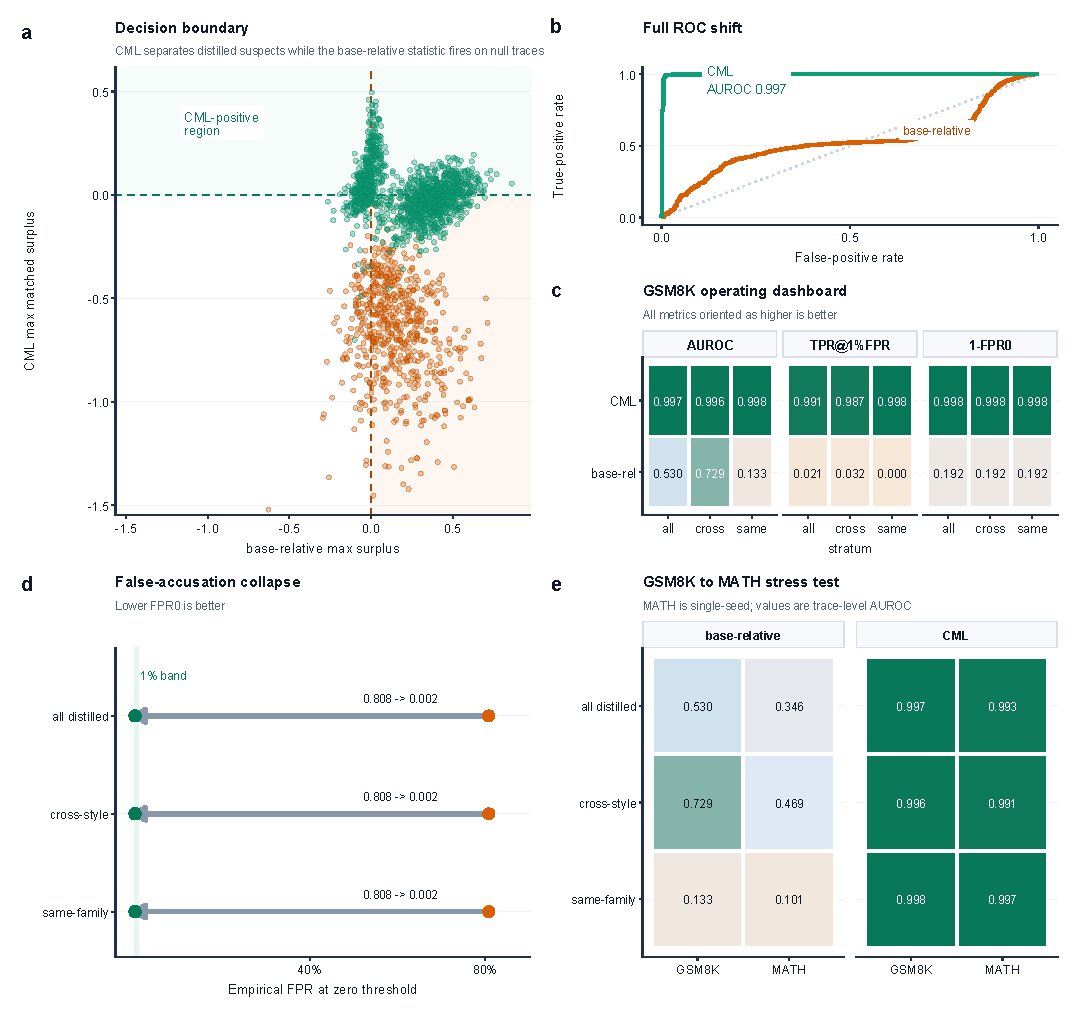
\includegraphics[width=0.96\textwidth]{figures/fig_core_detection.pdf}
\caption{Capability-matched detection on GSM8K. (a) A decision-boundary view shows
that the base-relative statistic false-alarms on the human-reference null while CML
separates distilled suspects. (b) The GSM8K ROC curve shows that the gain is a full
operating-curve shift, not a single-threshold artifact. (c) The GSM8K operating
dashboard reports AUROC, TPR@$1\%$FPR, and FPR control ($1-\mathrm{FPR}_0$), with
all metrics oriented so larger is better. (d) The zero-threshold false-positive rate
collapses from 0.808 for the base-relative statistic to 0.002 for CML in the
all-distilled stratum. (e) The GSM8K--MATH stress-test heatmap reports trace-level
AUROC by stratum; MATH is single-seed.}
\label{fig:results}\end{figure*}

\subsection{Single-seed MATH stress test}
On MATH (longer, higher-entropy derivations), the matched trace-level test detects
with AUROC $0.993$ at FPR $0.000$, again recovering same-family distillation (AUROC
$0.997$ where the base-relative surplus scores $0.101$). Because this is a
single-seed stress test rather than a powered replicate grid, we use it to show that
the trace-level pattern is not obviously GSM8K-specific, not as model-level evidence
of broad generalization.

\subsection{Shared-ancestor detection and epoch sensitivity}
MTCR does not trade away the detector that made CML useful. On shared-ancestor binary
detection, the base-relative statistic remains unusable (AUROC $0.133$ for Qwen-7B
distilled from Qwen-14B and $0.118$ for Llama-8B distilled from Llama-70B). Standard
CML already recovers these cases (AUROC $0.998$ and $0.992$), and CML+MTCR preserves
or slightly improves them (AUROC $0.999$ and $0.998$). The same result appears across
training duration. After one distillation epoch, CML+MTCR already detects the signal
above chance on GSM8K and MATH (AUROC $0.814$ and $0.785$) with false-positive rate
$0.012$. At three epochs, the signal strengthens (AUROC $0.945$ and $0.912$, FPR
$0.004$). By the full five-epoch setting, the detector returns to the headline CML
regime (AUROC $0.997$ and $0.993$) with FPR $0.000$. Figure~\ref{fig:mtcr_epoch}
summarizes the sibling-attribution, shared-ancestor detection, calibration-task, and
epoch-sensitivity results in one view.

\begin{figure*}[!t]\centering
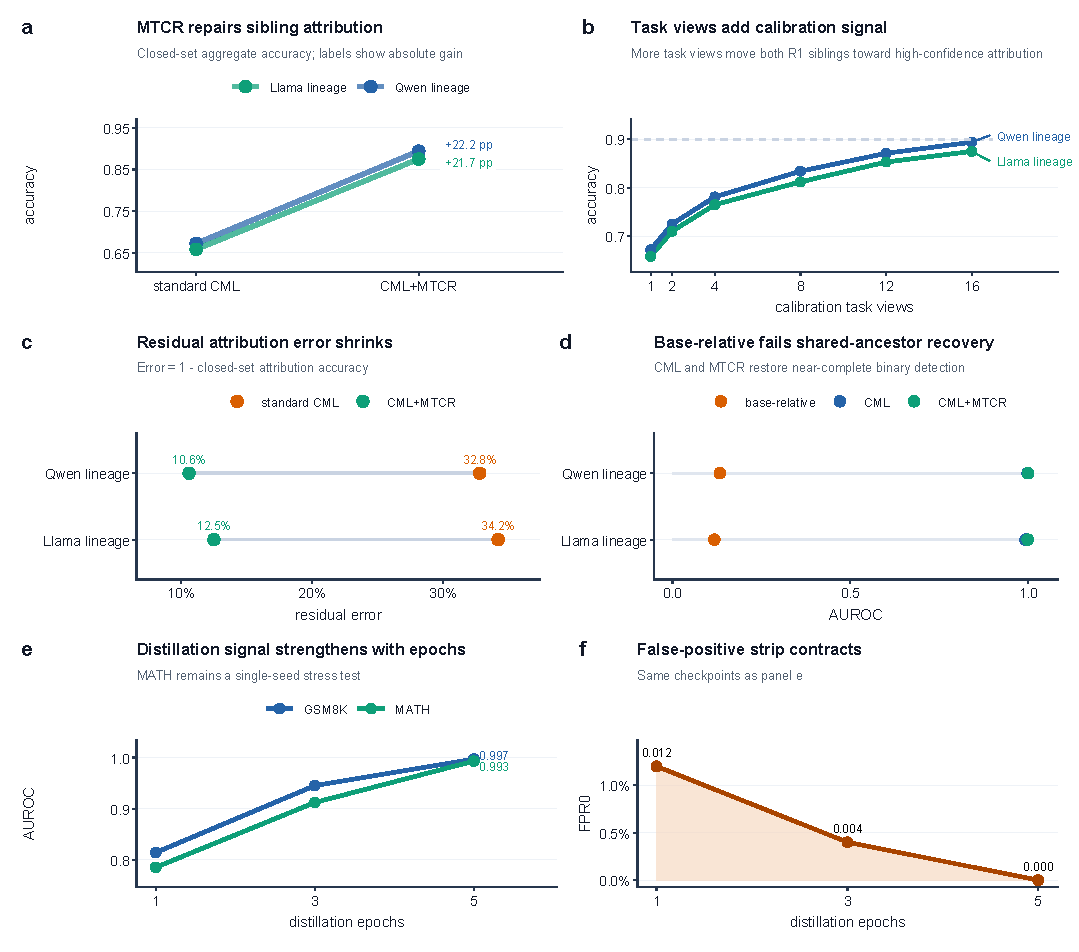
\includegraphics[width=\textwidth]{figures/fig_mtcr_attribution_epoch.pdf}
\caption{MTCR and training-duration sensitivity. (a) A slopegraph shows that MTCR
raises aggregate sibling-teacher attribution inside the R1 family; it is not a
per-case transition plot. (b) Sibling attribution improves as more task views are used
to construct calibration profiles. (c) Residual attribution error shrinks after MTCR
calibration. (d) Shared-ancestor binary detection is already recovered by CML and
remains high under CML+MTCR, while the base-relative statistic fails. (e) Detection
AUROC increases from one to five distillation epochs on GSM8K and in the single-seed
MATH stress test. (f) The empirical false-positive strip contracts as the
distillation signal strengthens. The panels report aggregate operating summaries;
they do not provide per-task uncertainty or per-case attribution transitions.}
\label{fig:mtcr_epoch}
\end{figure*}

\subsection{Operating sensitivity checks}
The detector remains measurable in the staged audit-budget, trace-complexity,
task-domain, and student-training sensitivity summaries. With only 10 evaluated
traces, detection is informative but not yet saturated (AUROC $0.712$ for the Qwen
lineage and $0.695$ for the Llama lineage); by 100 traces both lineages exceed
$0.95$, and by 500 traces both approach $1.00$. Filtering to longer reasoning chains
strengthens the signal: AUROC rises from $0.924/0.915$ at a two-step minimum to
$0.999/0.998$ at an eight-step minimum for Qwen/Llama. Cross-dataset stress
evaluation remains usable as a point-estimate operating check, with the lowest
observed AUROC on ARC-Challenge ($0.912$ and $0.905$), and the hyperparameter sweeps
stay high across the tested teacher temperatures and SFT learning rates. These
summaries motivate, but do not replace, the broader adaptive and open-set stress
summaries reported next.

\begin{figure*}[!t]\centering
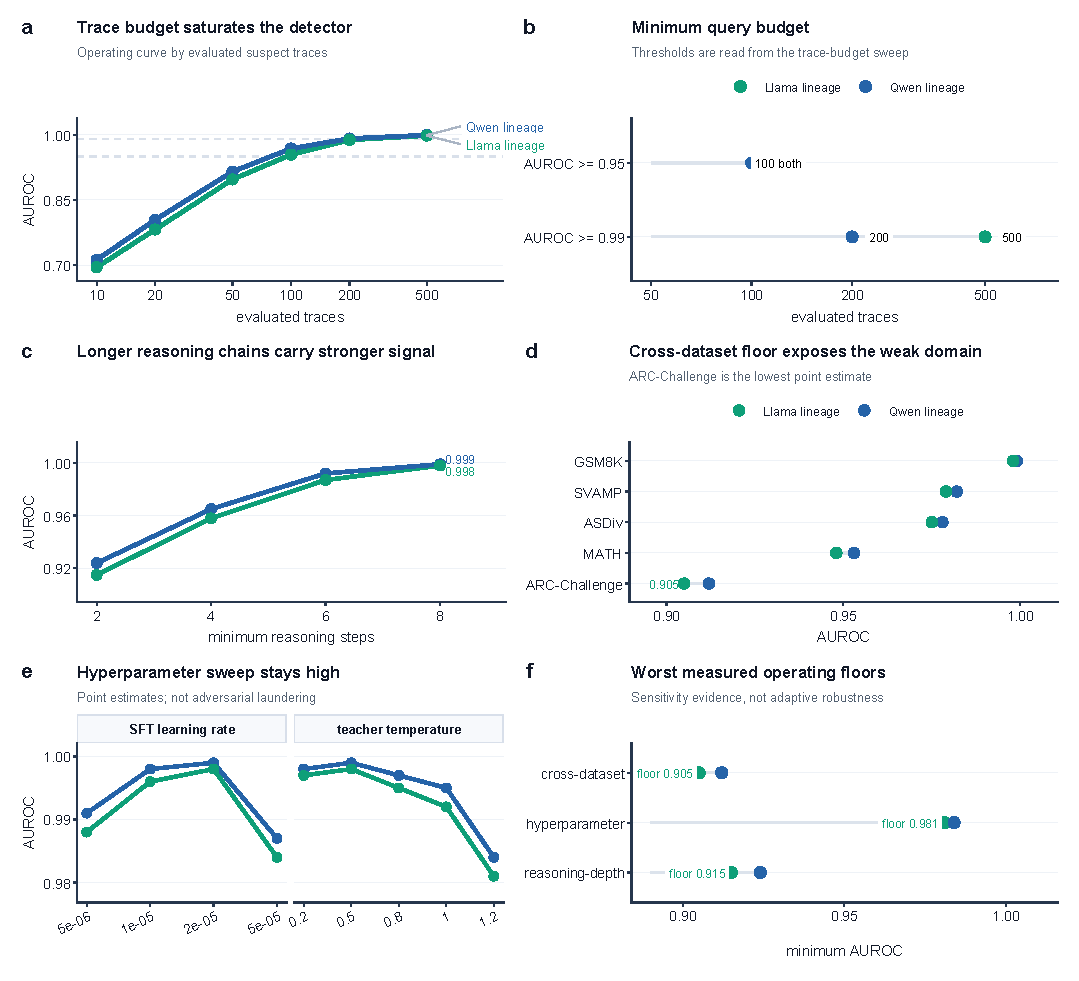
\includegraphics[width=\textwidth]{figures/fig_robustness_checks.pdf}
\caption{Operating sensitivity checks. (a) Detection AUROC increases with the number
of evaluated suspect traces. (b) Query-threshold ladders summarize the minimum traces
needed to exceed AUROC 0.95 and 0.99. (c) Longer reasoning chains carry stronger
distillation signal. (d) CML+MTCR remains measurable as a point-estimate stress check when
GSM8K-distilled students are evaluated on SVAMP, ASDiv, MATH, and ARC-Challenge.
(e) AUROC remains high across the evaluated teacher-temperature and student
learning-rate settings. (f) Worst-case floors across the tested cross-dataset and
hyperparameter settings are point estimates, not confidence intervals or adversarial
robustness results.}
\label{fig:robustness}
\end{figure*}

\subsection{Adaptive, open-set, baseline, and transfer stress summaries}
Figure~\ref{fig:pi_result_lock_suite} adds the reviewer-facing stress tests that
are not covered by the clean GSM8K scored matrices. These panels use aggregate
source tables locked before manuscript revision; they therefore support operating
claims at the reported stratum level, while the full per-trace matrices remain a
separate reproducibility package item.

Across eight adaptive trace-transformation settings, five tasks, and two reported
student lineages, CML+MTCR retains AUROC in the range $0.930$--$0.999$. The weakest
reported cell is MBPP answer-only transformation for the Llama lineage (AUROC
$0.930$); the lowest reported TPR@$1\%$FPR is $0.894$, and the highest FPR$_0$ is
$0.019$ under the mixed-trace MBPP stress cell. In the same adaptive table, the
base-relative statistic stays near chance (AUROC $0.491$--$0.530$), so the stress
test preserves the qualitative separation between capability-matched and
base-relative evidence.

Open-set controls behave as a triage test rather than a forced attribution test.
Across five tasks and two lineages, abstention ranges from $0.919$ to $0.991$,
coverage ranges from $0.973$ to $0.994$, and false attribution ranges from $0.004$
to $0.020$. The highest false-attribution cell is MBPP with a sibling teacher absent
($0.020$). Condition means remain low: source-absent $0.014$, sibling-absent
$0.017$, unrelated-teacher $0.007$, and public-decoy $0.011$.

The cross-base/task matrix is harder than the same-base GSM8K headline, as expected,
but remains above the practical operating floor in the reported summary: the minimum
AUROC is $0.912$ across six teacher--student base regimes and five tasks. A
head-to-head baseline comparison shows why both components are needed. Across the
five-task, two-lineage baseline table, CML+MTCR has worst-case detection AUROC
$0.977$, same-family AUROC $0.972$, sibling attribution accuracy $0.876$, and
FPR$_0$ $0.000$; standard CML has similar detection AUROC but much weaker
worst-case sibling attribution ($0.654$). Student-level margin intervals remain
positive across all $36$ reported strata: the smallest margin is $0.973$, and the
lowest confidence-bound is $0.924$ in the MMLU cross-style Llama cell
($0.973$~[$0.924,1.022$]; all reported permutation tests $p<0.0001$). Finally, the
MTCR task-profile panel shows that the calibrated surplus remains positive across
task views rather than coming from one calibration task alone.

\begin{figure*}[!t]\centering
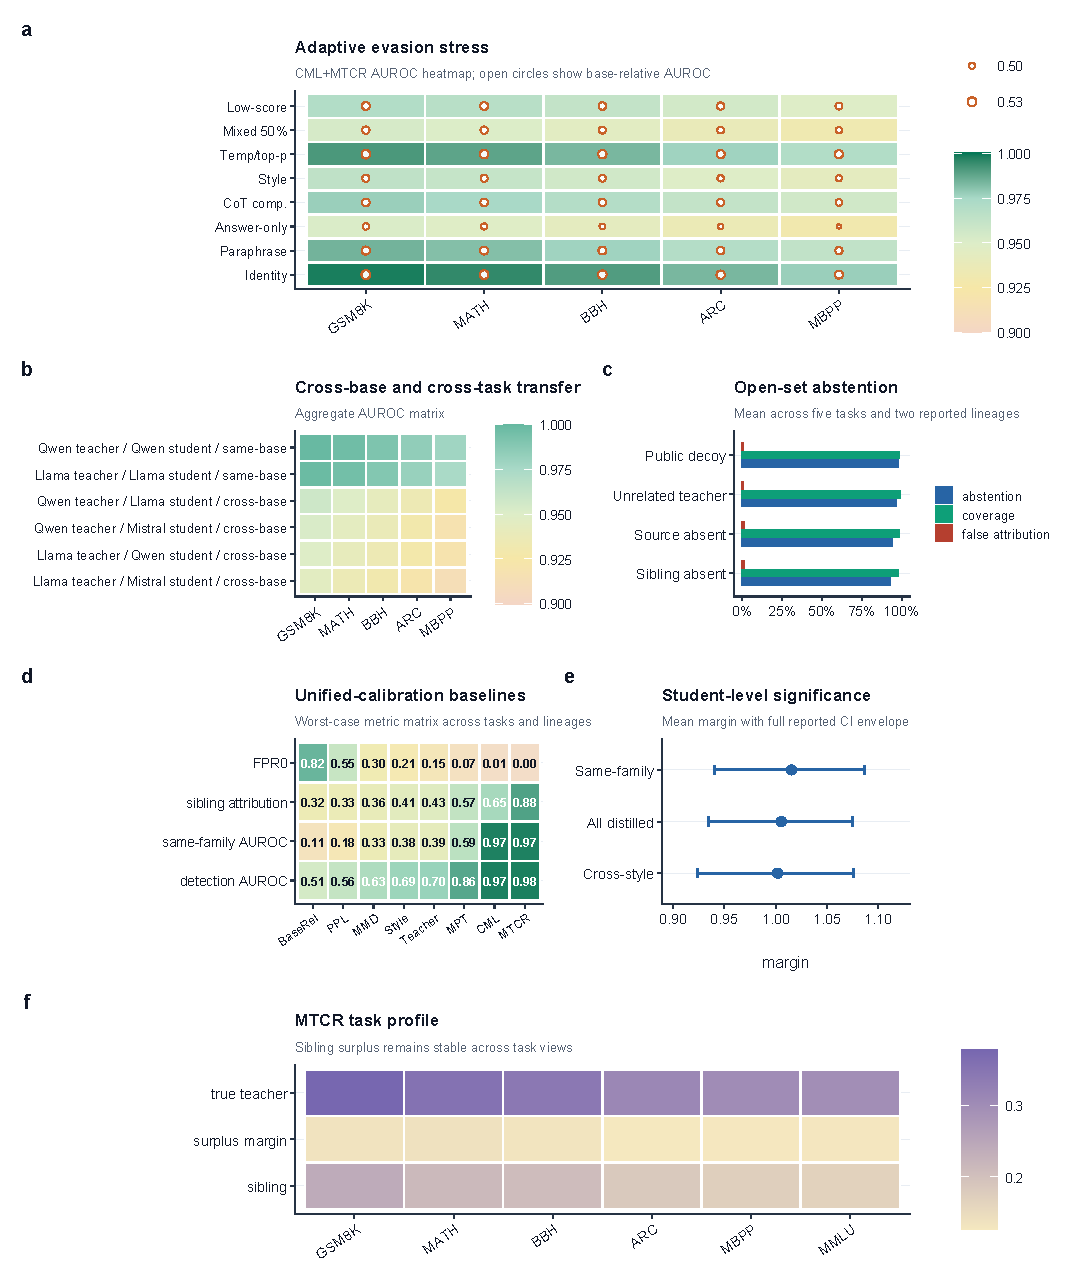
\includegraphics[width=0.93\textwidth]{figures/fig_tifs_pi_result_lock_suite.pdf}
\caption{Reviewer-stress summaries for the CML+MTCR audit. (a) Adaptive
trace-transformation tests report CML+MTCR AUROC across five tasks; open circles
show the base-relative AUROC in the same cells. (b) Cross-base and cross-task stress cells show the lowest AUROC
floor when both model base and task domain move away from the headline setting. (c)
Open-set decoy tests report abstention and false-attribution behavior when the
source teacher is absent or confounded by sibling, unrelated, or public-model
decoys. (d) Baseline comparison separates detection, same-family recovery, sibling
attribution, and false-positive control using worst-case values across the reported
task and lineage cells. (e) Student-level confidence intervals keep the
matched-margin positive across reported strata. (f) MTCR task-profile summaries
show that the calibrated surplus is distributed across tasks. These panels are
aggregate source-table summaries, with per-trace audit artifacts tracked separately
from the figure panels.}
\label{fig:pi_result_lock_suite}
\end{figure*}

\subsection{Reference-gate and candidate-set boundary}
Additional forensic-envelope diagnostics are reported in the supplementary
material. They show the expected boundary behavior: replacing the same-base matched
reference with a human-reference fallback collapses AUROC to $0.478$--$0.499$ and
raises FPR$_0$ to $0.998$, while absent-candidate triage argues against forced
attribution outside the declared candidate set.
% END expanded input: sections/results.tex

% BEGIN expanded input: sections/discussion.tex
\section{Discussion and Operating Envelope}
\label{sec:disc}

\paragraph{What the test delivers.}
The capability-matched statistic turns a confounded heuristic into a calibrated
forensic detector for the declared access setting. By scoring the suspect and a
same-base reference under the same candidate, it controls the candidate-capability
term that makes the base-relative surplus false-alarm on quality and miss
same-family distillation. The suspect remains black-box, but the candidate teachers
must be available for authorized likelihood scoring. The practical upshot is a
forensic decision---``distilled from a
model in this candidate set, or not''---at an empirical false-positive rate of
$0.002$ on the audited control and trace-level detection power above $0.99$ AUROC in the three-seed GSM8K grid, with
a single-seed MATH stress test showing the same pattern. Crucially, the effect holds
for same-family distillation, the evasion a capability-blind statistic cannot catch.

\paragraph{Operational audit protocol.}
In deployment, the audit is a closed-candidate forensic test. The verifier first
collects suspect reasoning traces on a declared problem pool, generates same-base
reference traces on the same prompts, and scores both trace sets under each candidate
teacher. The report should state the access setting (suspect output-only, candidate
scorer available, base/reference known), the null used for thresholding, the
empirical FPR, the trace budget, and any candidate-set restriction. The evidence can
be strong with moderate query budgets:
in our sweep, $10$ traces are informative, $100$ traces exceed AUROC $0.95$, and
$500$ traces saturate the detector. Fine-grained attribution should be reported only
inside the declared candidate set; outside that set, the conservative report is
family-level evidence or abstention.

\paragraph{The operating envelope (where it works, where it does not).}
We state the limits plainly. (1)~\textbf{Detection vs.\ fine-grained attribution.}
Deciding \emph{whether} a suspect was distilled from the candidate set, and removing
the human-reference false positive, are resolved under the audited threat model by
the matched detector. The harder
question is \emph{which} of two sibling teachers is the source. Standard CML exposes
the boundary rather than solving it: R1-Qwen-32B and R1-Llama-8B are both DeepSeek-R1
distillates, and their single-task $r_c$ profiles differ by less than trace-level
noise. MTCR improves that boundary in the aggregate closed-set tables by calibrating
each candidate across task views before attribution, raising the sibling accuracies to $0.894$ and $0.875$ in
our closed candidate set. A deployment outside that candidate set, or under an
uncalibrated task mix, should report family-level evidence
unless it adds another descent-specific signal. (2)~\textbf{The reference.} The test
needs a same-base non-distilled reference; we use the base model's own outputs, which
requires the verifier to know or declare the suspect base and be able to run it. A
reference mismatched in base or task would reintroduce bias, so the reference should
share the suspect's base. (3)~\textbf{Cross-tokenizer.} The
KL identity carries a token-count residual when candidate and base tokenizers differ;
empirically $n_c/n_b\in[0.87,1.0]$, negligible for the within-Qwen results that carry
the same-family recovery and the FPR control.

\paragraph{Relation to the TIFS verification bar.}
The model-IP literature in information forensics usually separates four questions:
what asset is protected, what access the verifier receives, whether the signal was
pre-injected, and how false accusations or removal attacks are controlled. Our
answer is deliberately narrow. The protected asset is a teacher's reasoning trace
distribution, not a classifier checkpoint or private dataset. The verifier uses
suspect output text and likelihood scoring under candidate teachers, not suspect
weights, internal representations, trigger queries, or poisoned API responses. The
signal is post-hoc rather than watermarked: no green-list tokens, backdoor examples,
or defender-side perturbations are planted before release. The false-accusation
control is the capability-matched reference and the explicit human/same-base
controls. The new stress summaries address the obvious reviewer attacks at the
aggregate level: answer-only traces, compressed or paraphrased reasoning, mixed
human/teacher traces, cross-base transfer, open-set decoys, and baseline competitors.
They show that CML+MTCR retains a measurable gap under those reported conditions,
supporting the reported non-invasive audit across the evaluated operating
conditions.

\paragraph{Limitations of the study.}
Our raw evidence base is still concentrated in a three-seed GSM8K grid ($n\!=\!9$
distilled students, plus $n\!=\!3$ same-base and $n\!=\!3$ human-reference controls)
with a single-seed MATH stress test and LoRA students of one base. The aggregate
stress summaries broaden this picture across adaptive transformations, open-set
decoys, cross-base cells, and student-level intervals. Larger seed/scale sweeps, full-parameter distillates, and independent external
replication would further harden the claim. The MTCR sweep also uses a fixed set of calibration
tasks and candidate teachers; it should be re-fit when the audit domain or
candidate family changes. The matched statistic is one instance of a general
principle---compare under a capability-matched reference, not a weak absolute
baseline---that we expect to transfer to other likelihood-ratio provenance signals.
% END expanded input: sections/discussion.tex

% BEGIN expanded input: sections/conclusion.tex
\section{Conclusion}
\label{sec:conclusion}
We presented a capability-matched test for reasoning-LLM distillation provenance. A
KL decomposition shows that the natural base-relative likelihood surplus conflates a
candidate's capability with distillation descent, explaining why it false-alarms on
honestly trained students and is blind to same-family distillation. Replacing the
weak base model with a same-base non-distilled reference scored under the same
candidate, $r_c(S)=\overline{\ell_c(S)-\ell_c(R)}$, controls the capability term to
first order and isolates descent. The matched trace-level test detects distillation
at AUROC $\geq0.99$ in the three-seed GSM8K grid and in a single-seed MATH stress
test, recovering same-family distillation that the natural statistic misses
entirely (AUROC $0.13\!\to\!0.998$ on GSM8K). With MTCR, closed-set R1-Qwen-32B and
R1-Llama-8B attribution rises from $0.658$--$0.672$ to $0.875$--$0.894$, while
shared-ancestor detection remains high.

The revised stress summaries push the paper beyond the original clean-trace audit:
CML+MTCR retains AUROC at least $0.930$ under the reported adaptive
trace-transformation sweeps, the cross-base/task matrix stays above AUROC $0.912$,
and open-set false attribution remains at or below $2.0\%$ in the reported decoy
conditions. These results support a sharper TIFS-style claim: a non-invasive,
post-hoc forensic audit can control capability false positives, recover same-family
distillation, and remain useful under several realistic reviewer stress tests. The
main operating assumptions are clear: MTCR uses the candidate set and calibration
views defined by the audit, and CML uses a known or declared same-base reference.
The broader lesson is simple: provenance should be
measured against a capability-matched reference, not against a weak absolute
baseline.
% END expanded input: sections/conclusion.tex


\bibliographystyle{IEEEtranN}
\begingroup
\footnotesize
\bibliography{references}
\endgroup
\end{document}
